\documentclass[conference]{IEEEtran}

\usepackage{cite}
\usepackage{amsmath,amssymb,amsfonts}
\usepackage{algorithmic}
\usepackage{graphicx}
\usepackage{textcomp}
\usepackage{xcolor}
\usepackage{booktabs}
\usepackage{siunitx}
\usepackage{float}
\usepackage[hidelinks]{hyperref}

%================  CUSTOMIZATION  =================================================%

\def\BibTeX{{\rm B\kern-.05em{\sc i\kern-.025em b}\kern-.08em
    T\kern-.1667em\lower.7ex\hbox{E}\kern-.125emX}}

\sisetup{
  detect-all,       % matches the surrounding font
  separate-uncertainty = true,
  per-mode = symbol  % m/s instead of m s^-1
}

\graphicspath{{Figures/}{../Common_assets/}}

% Generic upright subscript macros
\newcommand{\Ax}[1]{A_\mathrm{#1}}
\newcommand{\Ix}[1]{I_\mathrm{#1}}
\newcommand{\Px}[1]{P_\mathrm{#1}}
\newcommand{\Rx}[1]{R_\mathrm{#1}}
\newcommand{\rx}[1]{r_\mathrm{#1}}
\newcommand{\Vx}[1]{V_\mathrm{#1}}
\newcommand{\Zx}[1]{Z_\mathrm{#1}}
\newcommand{\gx}[1]{g_\mathrm{#1}}

%================  START OF DOCUMENT  =============================================%
\begin{document}

\title{Elektroniske enheter og kretser\\
Lab 05: Simulation of Operational Amplifier Configurations}

\author{\IEEEauthorblockN{Sølve Kjelseth}
\IEEEauthorblockA{\textit{Faculty of Technology, Natural Sciences and Maritime Sciences} \\
\textit{University of South-Eastern Norway}\\
Horten, Norway\\
274153@usn.no}
}

\maketitle

%================  ABSTRACT  ======================================================%

\begin{abstract}
This report presents simulation results for the operational amplifier LM358 and an instrumentation amplifier constructed from it.
Both inverting and non-inverting amplifier configurations were designed using calculated resistor values and simulated to verify theoretical gain relationships.  
Transient analysis was performed to verify the simulated voltage waveforms against theoretical predictions, while DC operating-point simulations confirmed correct biasing and expected voltage levels.

An instrumentation amplifier using three LM358 devices was then implemented to demonstrate its ability to amplify a small differential signal while rejecting a large common-mode component.  
The transient results show high accuracy in isolating the signal of interest, with simulated gains closely matching the calculated values.  
\end{abstract}

%================  KEYWORDS  ======================================================%
\begin{IEEEkeywords}
operational amplifier, LM358, inverting amplifier, non-inverting amplifier, instrumentation amplifier
\end{IEEEkeywords}

%================  INTRODUCTION  ==================================================%
\section{Introduction}
% #region

Operational amplifiers are versatile components used in a wide range of analogue circuit applications.  
A solid understanding of their operating principles and common configurations is essential for circuit design and analysis.  
Simulation provides a convenient and reliable method for investigating amplifier performance under ideal and non-ideal conditions before building a physical circuit.

This report focuses on three fundamental amplifier configurations based on the LM358 operational amplifier: the inverting amplifier, the non-inverting amplifier, and the three-op-amp instrumentation amplifier.  
The first two serve to verify the basic gain equations and phase relationships through simulation, while the latter demonstrates differential signal amplification and common-mode rejection.  

Each circuit was designed using calculated resistor values to meet specified voltage-gain targets.  
Simulations were performed to evaluate both the transient response and DC operating points, enabling direct comparison with theoretical expectations.  
The results illustrate how practical amplifier behaviour aligns with analytical models and highlight the advantages of the instrumentation-amplifier topology in measurement applications.

All AC voltages discussed in this report refer to peak values.  
All operational amplifiers were powered from symmetric supply rails of \(\pm\qty{12}{\volt}\).

% #endregion


%================  SUBSECTION  ====================================================%
\subsection{Inverting amplifier design and simulation}
% #region

The first objective is to design and simulate an inverting operational amplifier using the LM358 model.  
This circuit demonstrates the characteristic phase inversion and precise gain control achieved through negative feedback.  
By comparing theoretical predictions with simulation results, the accuracy of the analytical model and the influence of practical device limitations can be evaluated.

To obtain a voltage gain of \(\Ax{V}=\qty{-20}{}\), an input resistor of \(\qty{1}{\kilo\ohm}\) was selected, giving a required feedback resistor of \(\qty{20}{\kilo\ohm}\) according to (\ref{eq:invgain}).  

Assuming a theoretical output amplitude of \(\qty{10}{\volt}\), the input voltage was calculated from (\ref{eq:voinv}).  
This results in an input signal of \(\qty{500}{\milli\volt}\) at \(\qty{1}{\kilo\hertz}\).  
An inverting amplifier theoretically exhibits a \(\qty{180}{\degree}\) phase shift between input and output due to its negative gain.

The schematic with simulated DC operating-point annotations is presented in Figure~\ref{fig:circuit1}.  
The operating point shows that the inverting input node is held close to the virtual ground, measured at \(\qty{2.0}{\milli\volt}\), established by the non-inverting input, verifying correct biasing of the LM358 model.  
The output DC offset is also small, at \(\qty{41.2}{\milli\volt}\).  

A transient analysis was then performed, and the resulting input and output waveforms are shown in Figure~\ref{fig:transinv}.  
Measurements were taken from the simulation to determine the gain and phase shift.  
A comparison between theoretical and simulated results is summarised in Table~\ref{tab:inv_results}.  
The excellent agreement indicates that non-ideal parameters such as input bias current and parasitic capacitors of the LM358 have negligible influence at \(\qty{1}{\kilo\hertz}\).  


\begin{equation}
\label{eq:invgain}
    \Ax{V} = - \frac{\Rx{f}}{\Rx{in}}
\end{equation}

\begin{equation}
    \label{eq:voinv}
    \Vx{o} = \Ax{V} \cdot \Vx{i}
\end{equation}

\begin{figure}[!t]
    \centering
    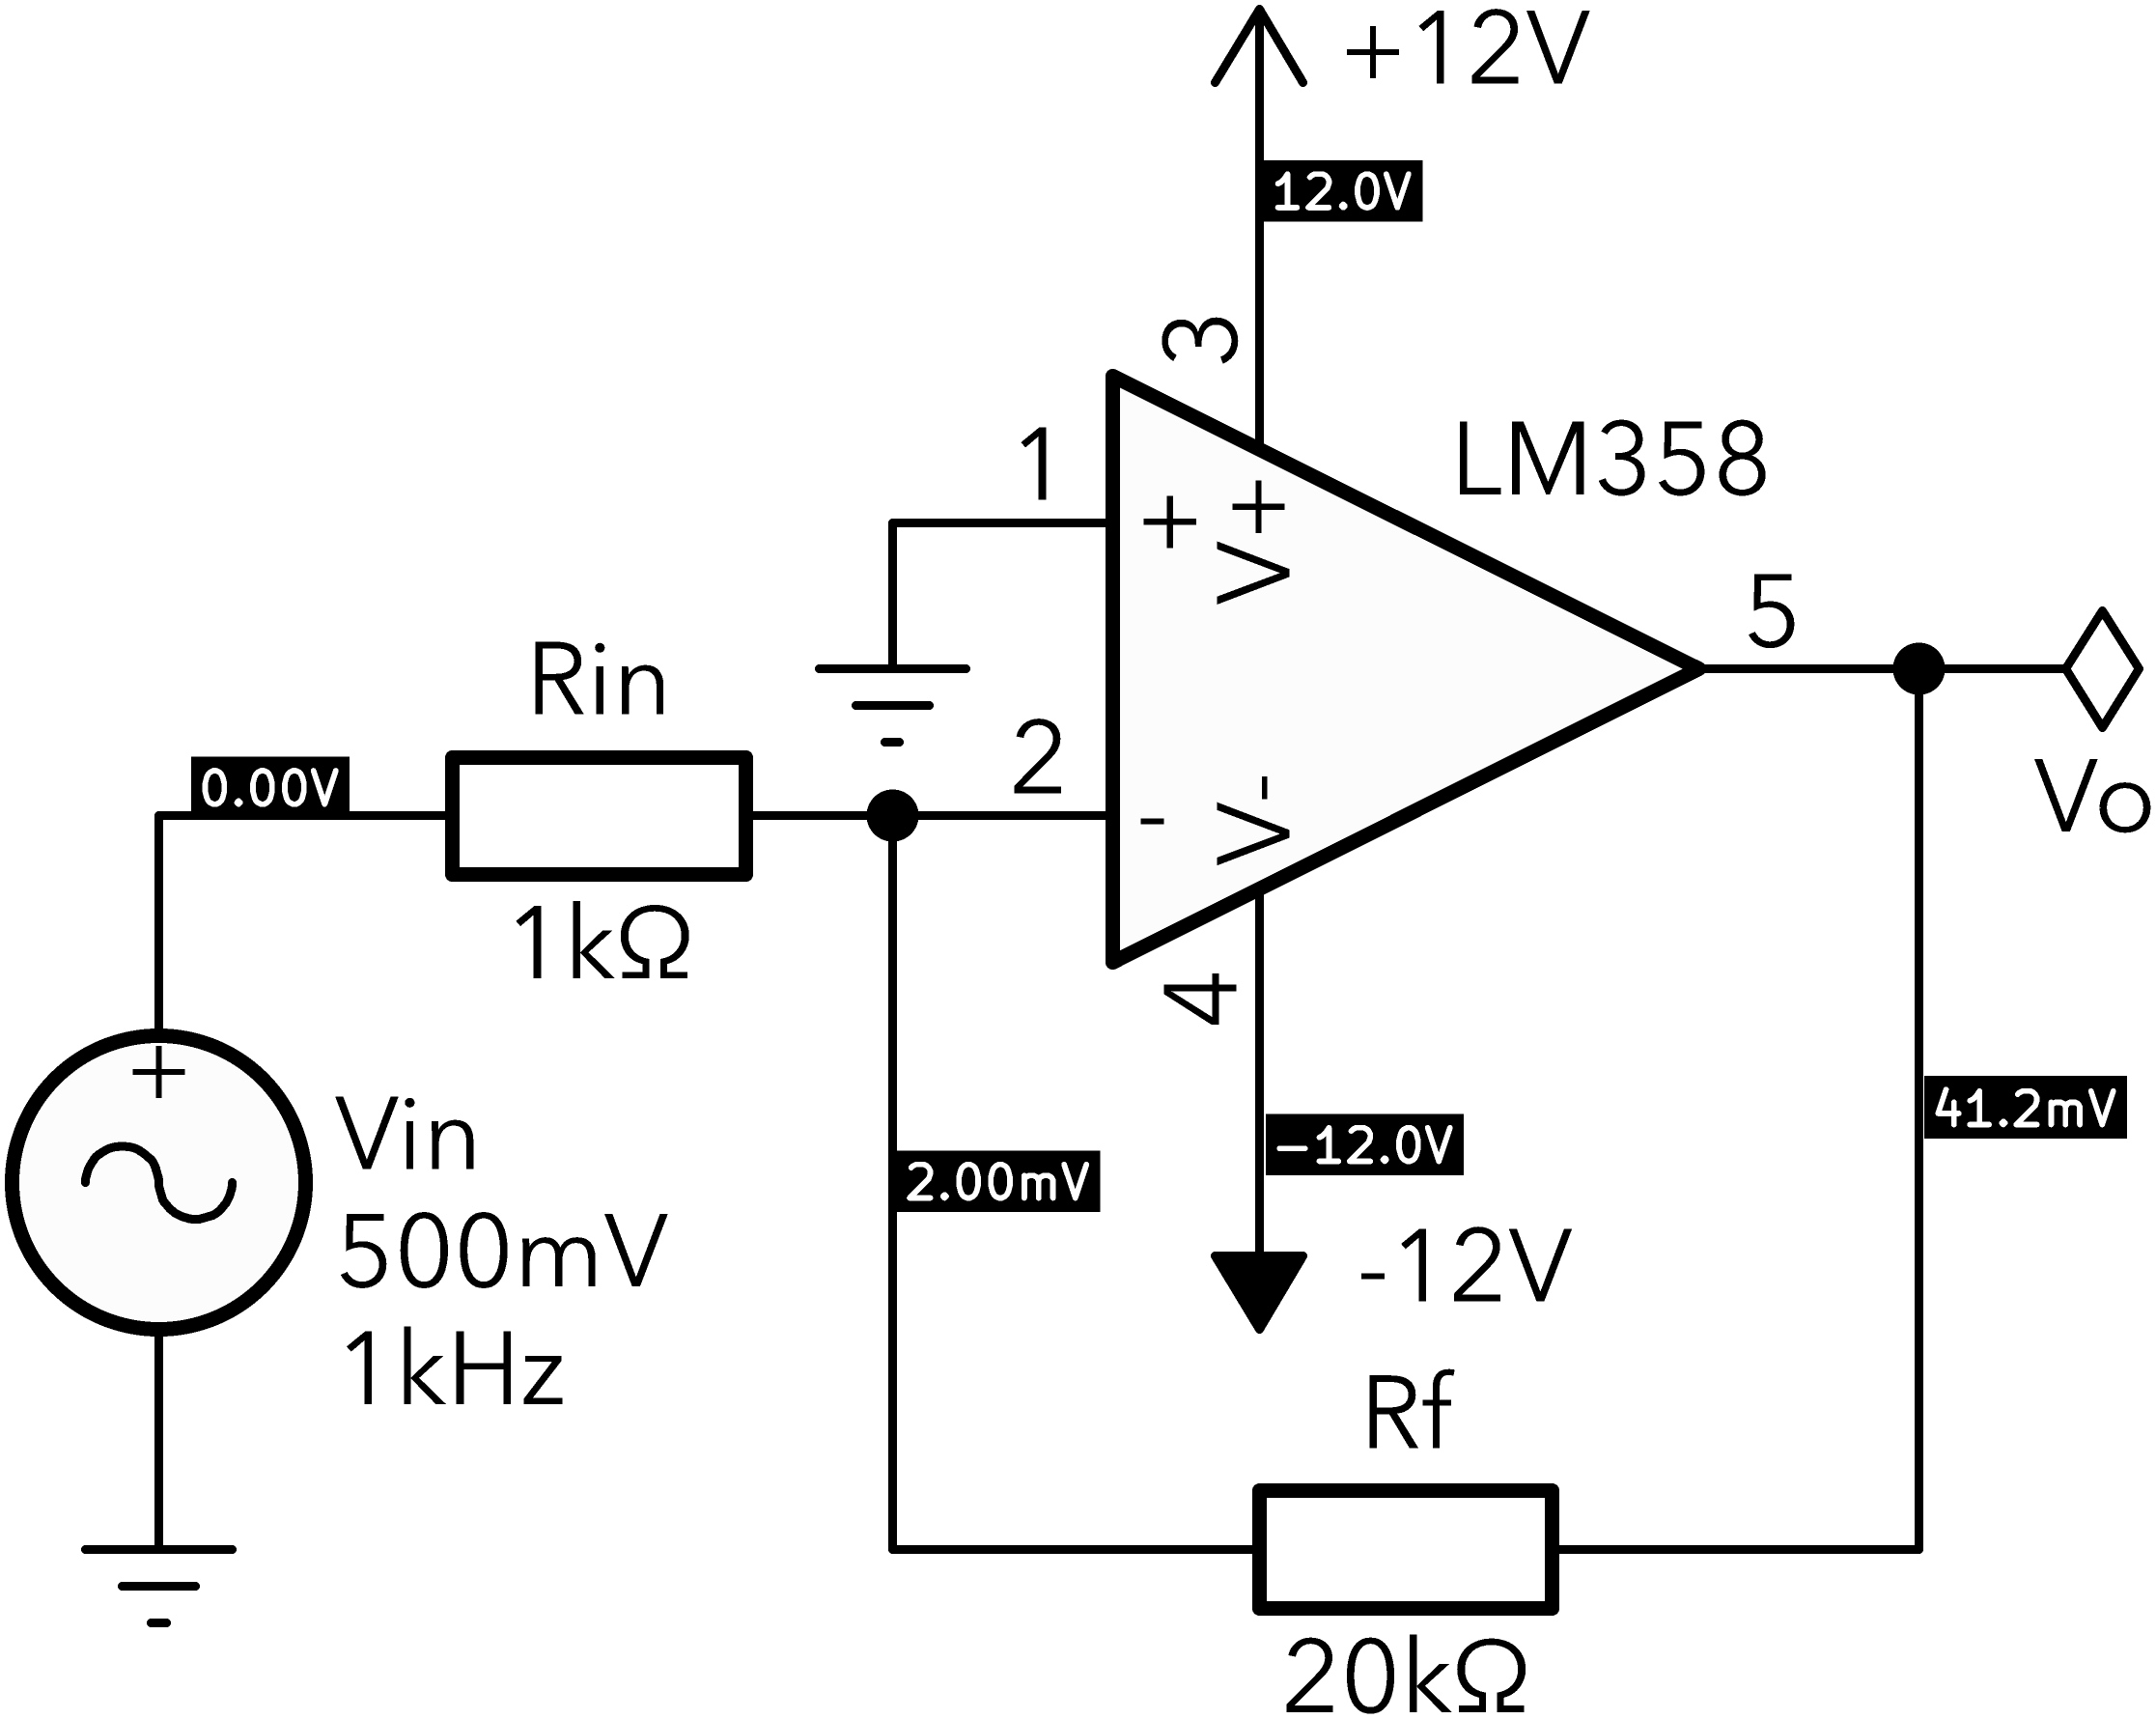
\includegraphics[width=0.9\linewidth]{SchematicInverting.jpg}
    \caption{Schematic of the inverting amplifier with DC operating points.}
    \label{fig:circuit1}
\end{figure} 

\begin{figure}[!b]
    \centering
    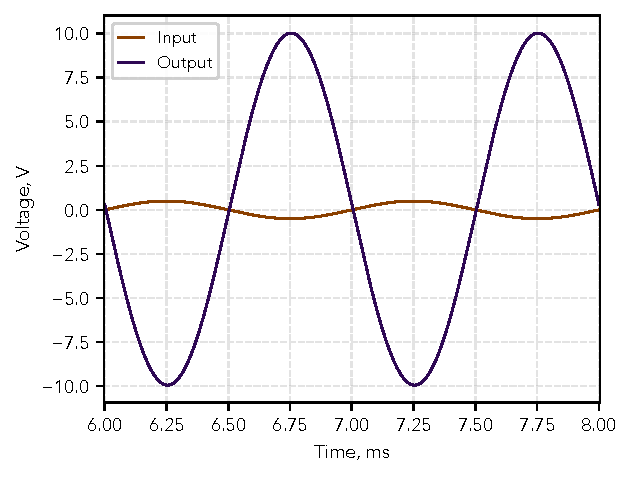
\includegraphics[width=0.9\linewidth]{TransientPlot_Inverting.pdf}
    \caption{Transient analysis showing waveforms of the inverting amplifier.}
    \label{fig:transinv}
\end{figure} 

\begin{table}[!b]
    \centering
    \caption{Comparison of theoretical and simulated results}
    \label{tab:inv_results}
    \begin{tabular}{l S[table-format=4.3] S[table-format=4.3] l}
        \toprule
        Parameter & {Theoretical} & {Simulated} & Unit \\
        \midrule
        \(\Vx{o}\)      & 10.000  & 10.036  & \(\unit{\volt}\) \\
        \(\Ax{V}\)      & -20.00 & -20.07 & --- \\
        Phase shift     & 180.0   & 178.5   & \(\unit{\degree}\) \\
        \bottomrule
    \end{tabular}
\end{table}

% #endregion


%================  SUBSECTION  ====================================================%
\subsection{Non-inverting amplifier design and simulation}
% #region

The second objective is to design and simulate a non-inverting operational amplifier using the LM358 model.  
This configuration demonstrates high input impedance and provides positive voltage gain without phase inversion.  
By comparing theoretical and simulated results, the accuracy of the model can be evaluated.

To achieve a voltage gain of approximately \(\Ax{V}=\qty{40}{}\), a resistor \(\Rx{g}=\qty{1}{\kilo\ohm}\) was selected for the ground leg and a feedback resistor \(\Rx{f}=\qty{39}{\kilo\ohm}\) was calculated according to (\ref{eq:ninvgain}).  

\begin{equation}
\label{eq:ninvgain}
    \Ax{V} = 1 + \frac{\Rx{f}}{\Rx{g}}
\end{equation}

Assuming a desired output amplitude of \(\qty{8}{\volt}\), the corresponding input voltage was determined from (\ref{eq:voinv}).  
This gives an input signal of \(\qty{200}{\milli\volt}\) at \(\qty{1}{\kilo\hertz}\).  
As the gain is positive, the theoretical phase shift between input and output is \(\qty{0}{\degree}\).

The simulated schematic with DC operating-point annotations is shown in Figure~\ref{fig:circuit2}.  
The results confirm correct biasing of the LM358, with the non-inverting input near ground potential and a small output DC offset within the linear operating range of the amplifier.  

A transient analysis was performed to verify the AC behaviour, and the resulting waveforms are shown in Figure~\ref{fig:transnivn}.  
Measurements from the simulation were used to calculate the gain and phase shift.  
A comparison of theoretical and simulated values is summarised in Table~\ref{tab:ninv_results}.  
The close match confirms that the LM358 performs as expected at \(\qty{1}{\kilo\hertz}\), with only minor phase deviation of a few degrees caused by the finite gain-bandwidth product.  
This deviation is negligible for low-frequency applications where the closed-loop gain remains stable.

\begin{figure}[!b]
    \centering
    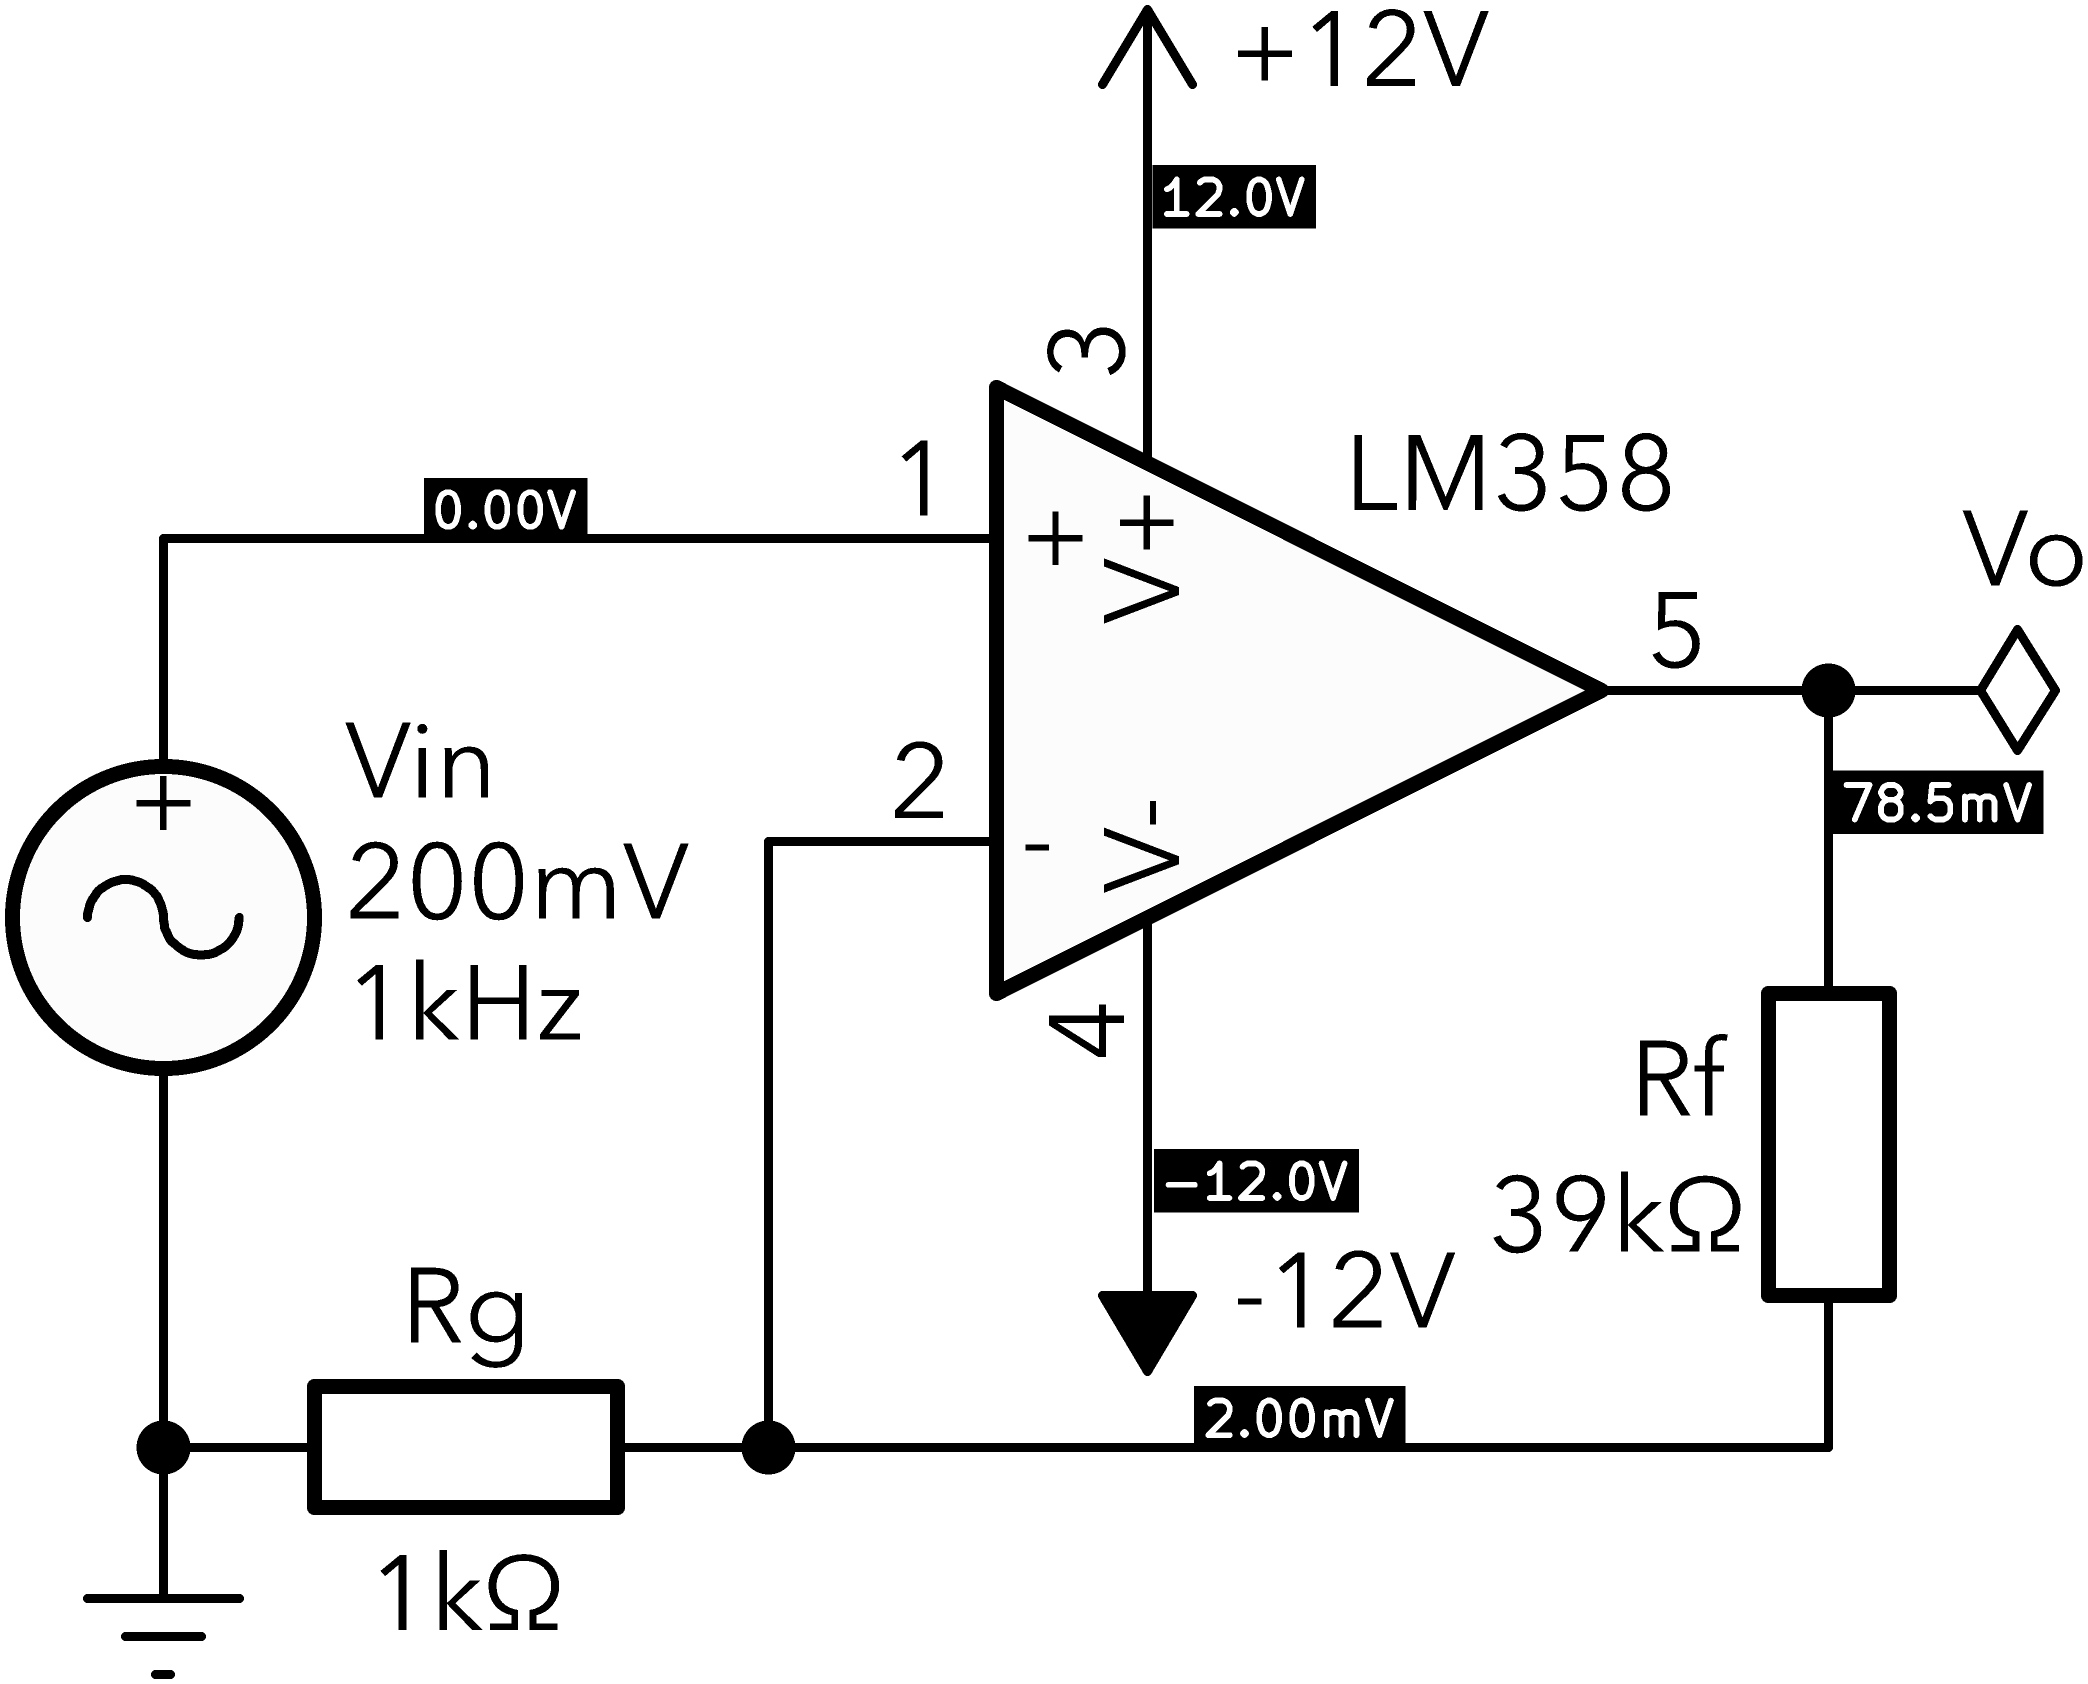
\includegraphics[width=0.8904\linewidth]{SchematicNonInverting.jpg}
    \caption{Schematic of the non-inverting amplifier with DC operating points.}
    \label{fig:circuit2}
\end{figure}

\begin{figure}[!t]
    \centering
    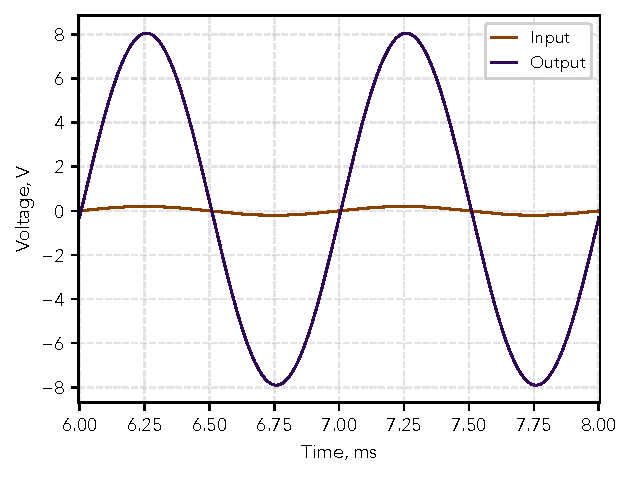
\includegraphics[width=0.9\linewidth]{TransientPlot_NonInverting.pdf}
    \caption{Transient analysis showing waveforms of the non-inverting amplifier.}
    \label{fig:transnivn}
\end{figure}


\begin{table}[!b]
    \centering
    \caption{Comparison of theoretical and simulated results}
    \label{tab:ninv_results}
    \begin{tabular}{l S[table-format=4.3] S[table-format=4.3] l}
        \toprule
        Parameter & {Theoretical} & {Simulated} & Unit \\
        \midrule
        \(\Vx{o}\)      & 8.000  & 8.066  & \(\unit{\volt}\) \\
        \(\Ax{V}\)      & 40.00  & 40.33  & --- \\
        Phase shift     & 0.0    & -2.9    & \(\unit{\degree}\) \\
        \bottomrule
    \end{tabular}
\end{table}


% #endregion

%================  SUBSECTION  ====================================================%
\subsection{Instrumentation amplifier design and simulation}
% #region


The final objective is to design and simulate a three-op-amp instrumentation amplifier using the LM358 model.  
This circuit demonstrates how differential amplification can be achieved while rejecting large common-mode signals.  
By comparing the theoretical and simulated results, the effectiveness of the design in isolating the small signal of interest can be evaluated.

The instrumentation amplifier was implemented with equal resistor values \(\Rx{1}=\Rx{2}=\Rx{3}=\Rx{4}=\qty{10}{\kilo\ohm}\), giving the second stage a unity gain according to (\ref{eq:stage2gain}).  
The two feedback resistors in the first stage were also set to \(\qty{10}{\kilo\ohm}\), with the gain determined by the resistor \(\Rx{G}\) as described by (\ref{eq:stage1gain}).  
To obtain a low overall gain and maintain a readable signal amplitude for the transient plot, a resistor \(\Rx{G}=\qty{3.3}{\kilo\ohm}\) was selected.  
This results in a theoretical first-stage gain of \(\Ax{V1}=\qty{7.06}{}\).

During simulation, the circuit was initially non-functional due to two wiring errors in the schematic—one affecting the first-stage feedback loop and the other the differential connection of the second stage.  
After correcting these issues, the amplifier performed as expected, illustrating the importance of schematic verification before simulation.

The schematic with DC operating-point annotations is shown in Figure~\ref{fig:circuit3}.  
A transient analysis was performed with a differential input consisting of a small signal superimposed on a large common-mode voltage.  
The resulting output waveform, shown in Figure~\ref{fig:transins}, clearly demonstrates that the output depends only on the differential input; the common-mode component is effectively suppressed. 

The simulated outputs were measured and is summarised and compared to calculations in Table~\ref{tab:instr_results}. 
The phase shift could not be measured accurately due to the large common-mode input but appeared close to \(\qty{0}{\degree}\), as theoretically expected.
The small deviation in gain is primarily due to resistor tolerances and the finite open-loop gain of the LM358.  
Nevertheless, the circuit successfully demonstrates the functionality and precision of an instrumentation amplifier configuration.

\begin{table}[!b]
    \centering
    \caption{Comparison of theoretical and simulated results}
    \label{tab:instr_results}
    \begin{tabular}{l S[table-format=4.3] S[table-format=4.3] l}
        \toprule
        Parameter & {Theoretical} & {Simulated} & Unit \\
        \midrule
        \(\Vx{o}\)      & 35.303  & 39.433      & \(\unit{\milli\volt}\) \\
        \(\Ax{V}\)      & 7.06    & 7.89        & --- \\
        Phase shift     & 0.0     & \approx 0 & \(\unit{\degree}\) \\
        \bottomrule
    \end{tabular}
\end{table}



\begin{figure}[!t]
    \centering
    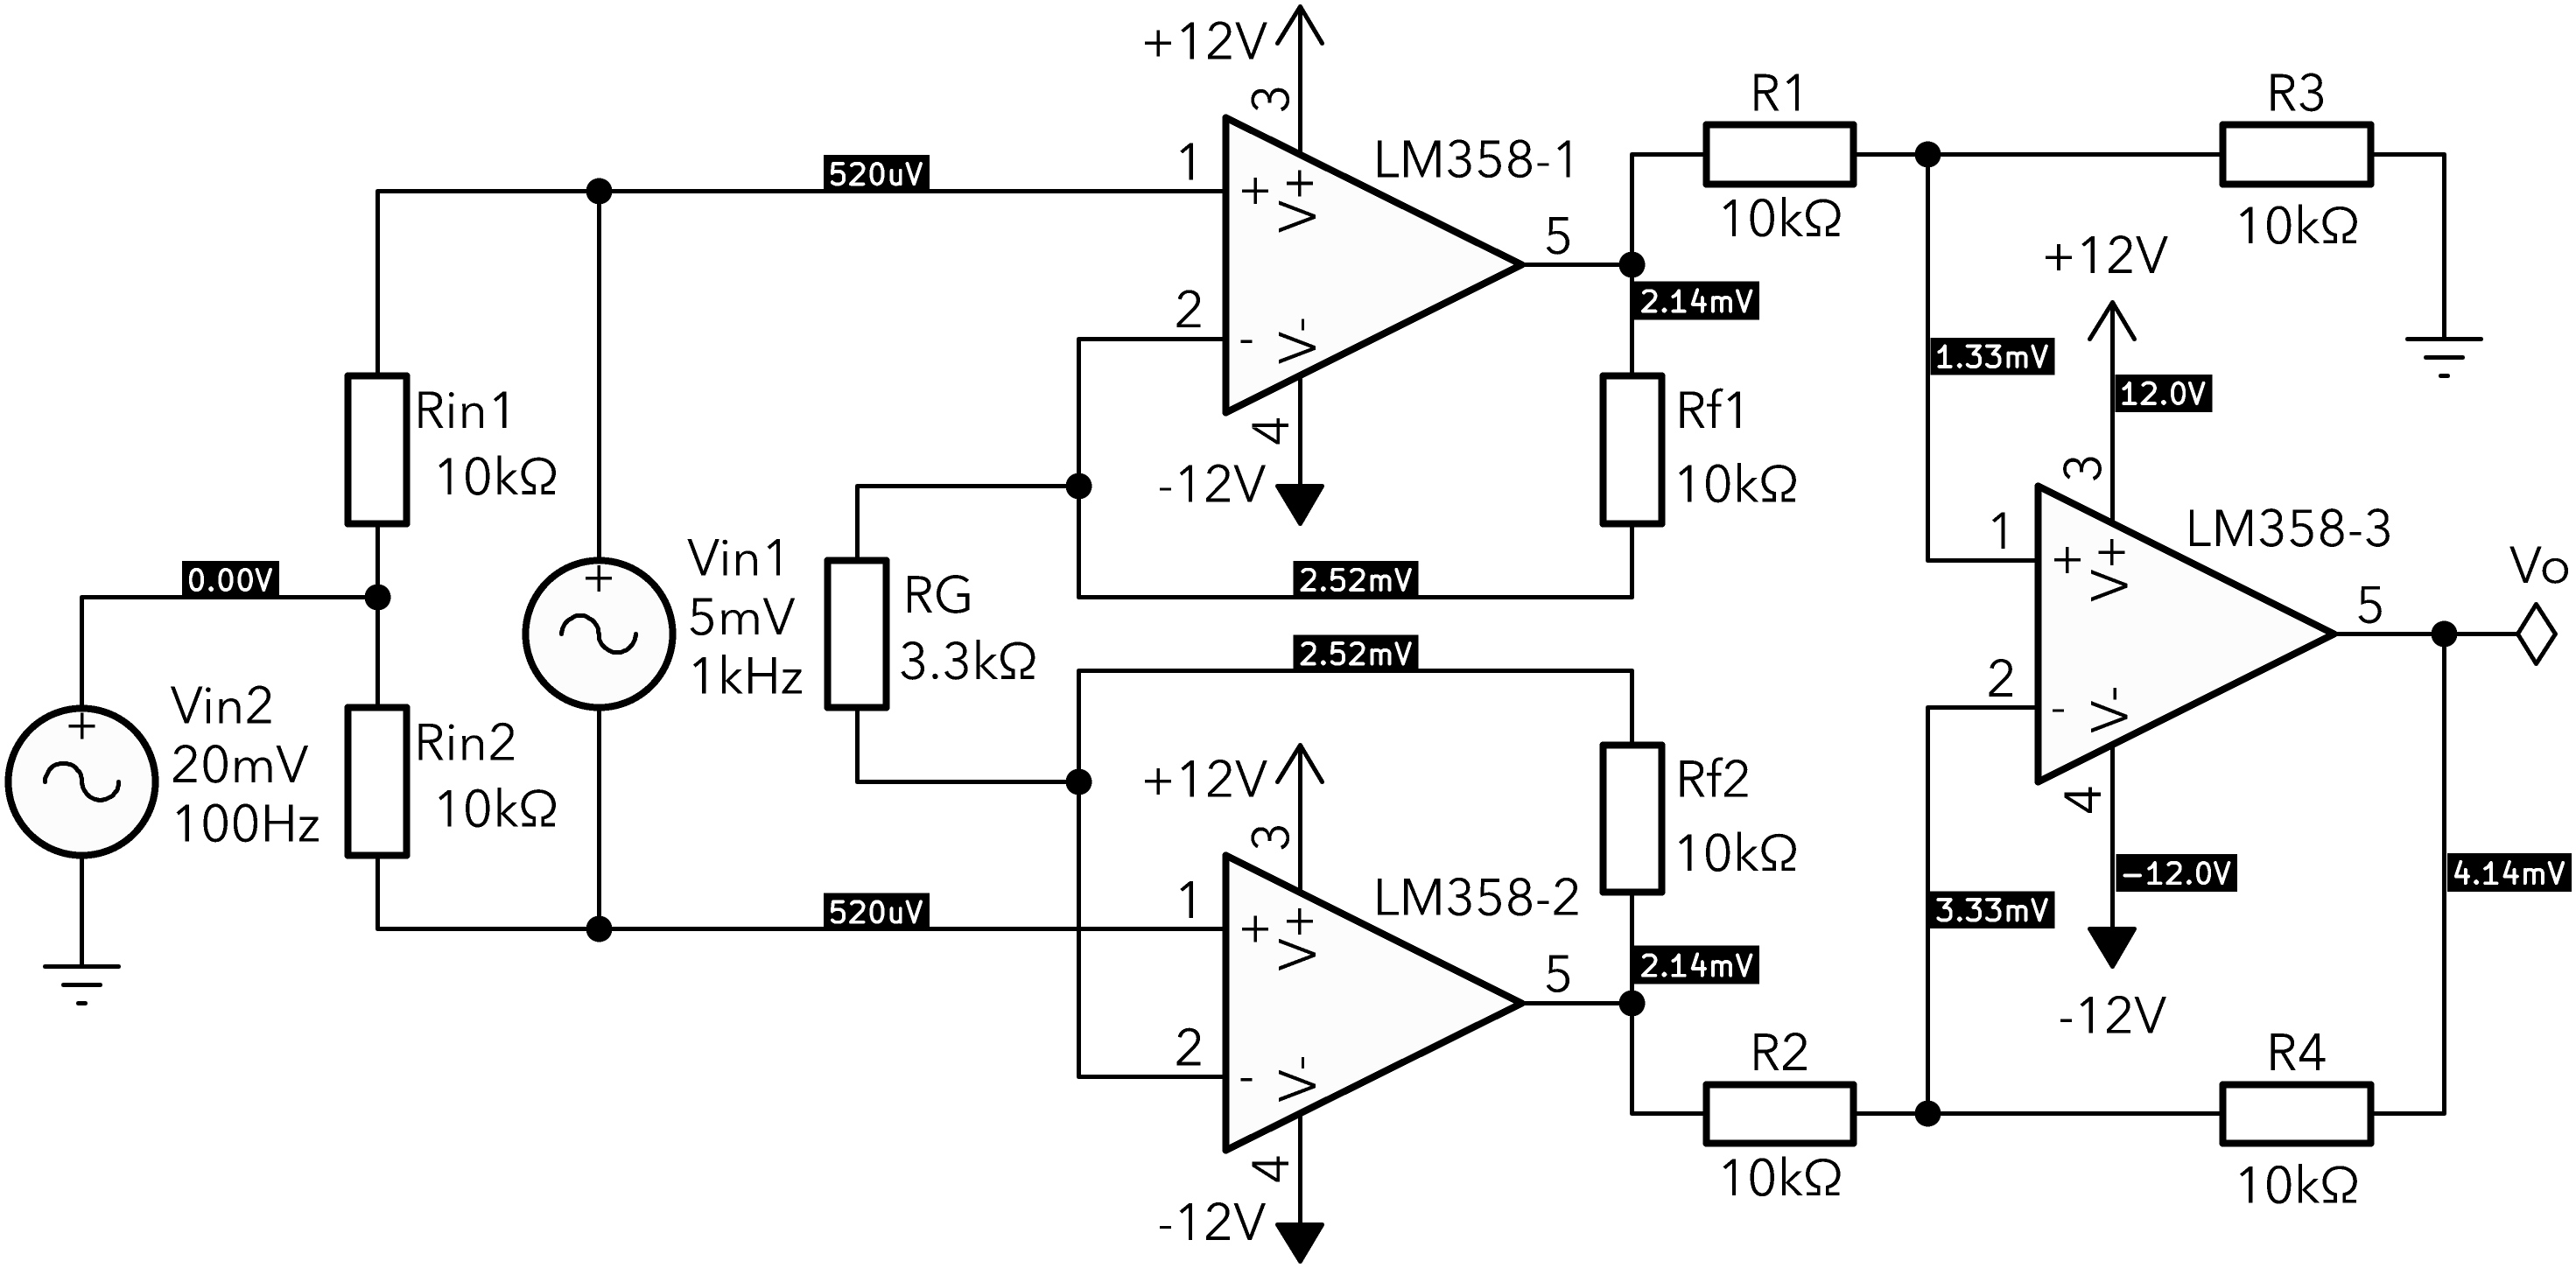
\includegraphics[width=0.9\linewidth]{SchematicIntrumentation.jpg}
    \caption{Schematic of the instrumentation amplifier with DC operating points.}
    \label{fig:circuit3}
\end{figure}

\begin{figure}[!t]
    \centering
    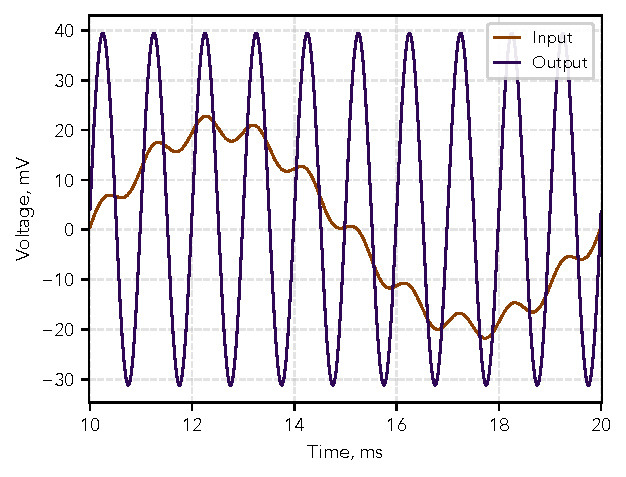
\includegraphics[width=0.9\linewidth]{TransientPlot_Instrumentation.pdf}
    \caption{Transient analysis showing waveforms of the instrumentation amplifier.}
    \label{fig:transins}
\end{figure}

\begin{equation}
\label{eq:stage2gain}
    \Ax{V2} = \frac{\Rx{2}}{\Rx{1}} = \frac{\Rx{4}}{\Rx{3}}
\end{equation}

\begin{equation}
\label{eq:stage1gain}
    \Ax{V1} = 1 + \frac{2 \cdot \Rx{f}}{\Rx{G}}
\end{equation}

Compared with a single operational amplifier in either inverting or non-inverting configuration, the instrumentation amplifier offers several advantages.  
Its differential input stage provides a very high input impedance and ensures that both input signals are referenced to the same impedance environment, minimising offset errors.  
More importantly, it achieves a high common-mode rejection ratio (CMRR), allowing accurate amplification of small differential signals in the presence of large common-mode voltages.  
This makes the design well suited for sensor and measurement applications, where signal integrity and precision are critical.




% #endregion


%================  CONCLUSION  ====================================================%
\section{Conclusion}
% #region

This report has presented the design and simulation of several operational amplifier configurations using the LM358 model.  
Both the inverting and non-inverting amplifiers achieved the expected gains of \(\qty{-20}{}\) and \(\qty{40}{}\), respectively, with simulated results closely matching theoretical calculations.  
DC operating-point analysis confirmed correct biasing and stable operating conditions for all circuits.  

The instrumentation amplifier successfully amplified a small differential signal while rejecting a large common-mode component, as expected from its circuit configuration.  
The small deviation between theoretical and simulated gain is most likely due to internal parasitic resistances and capacitances within the realistic LM358 model, which slightly affect the frequency response.  

During the instrumentation amplifier design, initial connection errors highlighted the importance of careful schematic verification prior to simulation.  
This experience reinforced good design practice and improved understanding of amplifier configuration and signal referencing.  

\newpage

Overall, the simulations verified the theoretical models of all amplifier types and provided practical insight into the behaviour and advantages of differential amplifier circuits.

% #endregion


%================  ACKNOWLEDGMENT  ================================================%
\section*{Acknowledgment}
% #region
This report corresponds to Lab~05 in the course \emph{Elektroniske enheter og kretser}.
All related materials (\LaTeX~sources, raw data, figures, codes and more) are released under the MIT License and available at \url{https://github.com/Kjelseth/EEK_lab}.
% #endregion

\end{document}